The Services page aims to show all the services provided by our association. In the page is possible to click on each service image or title to access to its dedicated page.

\begin{figure}[h!]
		\centering
		\begin{minipage}[b]{1\textwidth}
    			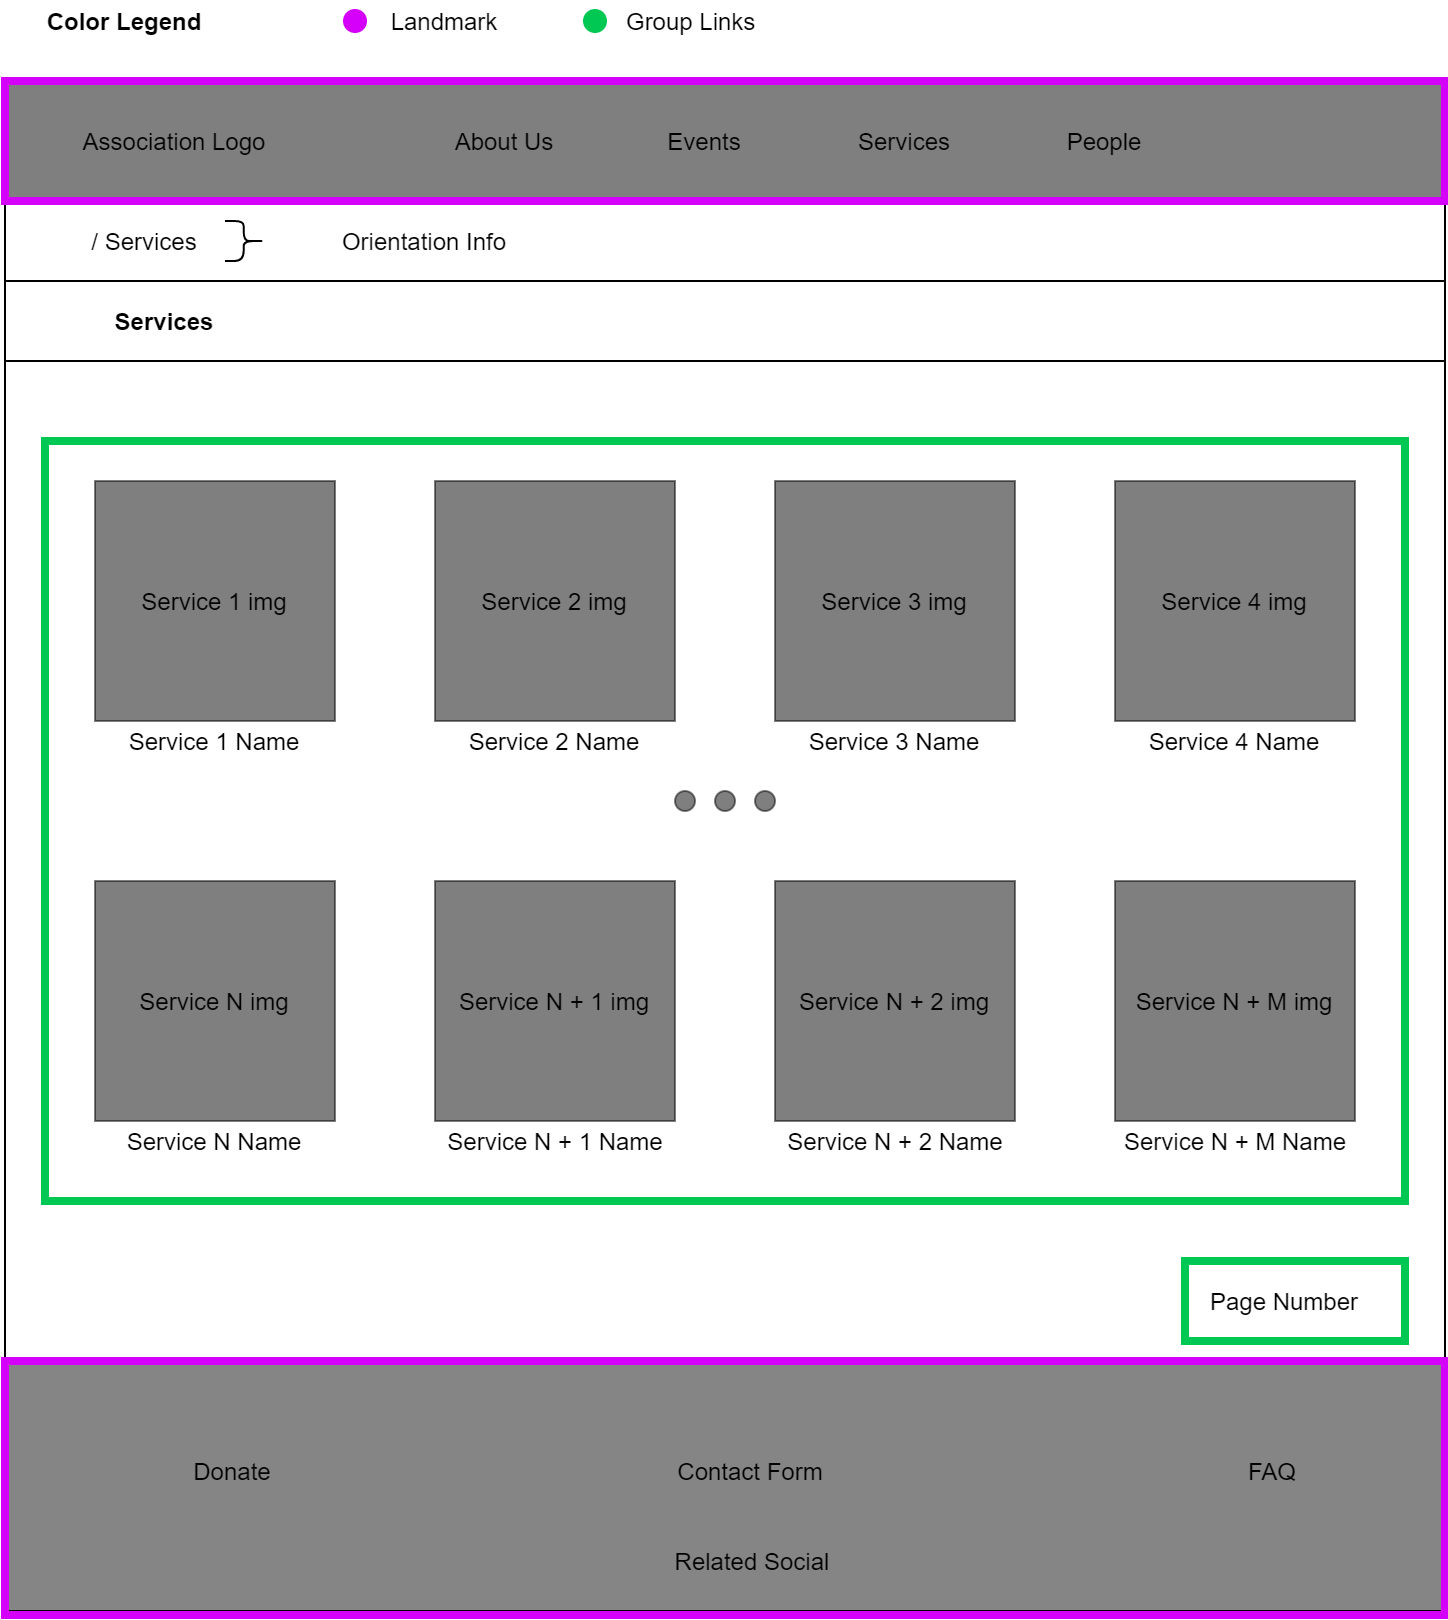
\includegraphics[width=\textwidth]{./assets/services.png}
			\caption{Services Page - Design in the small}
		\end{minipage}
	\end{figure}
\FloatBarrier
\vspace{1cm}
\hspace{-1cm}
Services' details can be found in Service page, which contains:
\begin{itemize}
	\item a carousel with all images related to the selected service, there must be at least one image and all of them are retrieved 			from the database;
	\item practical info and a brief description that explain the service purpose and all important information that users need;
	\item the transition links to the volunteer that are involved in the selected service;
	\item the transition links to the events in which the selected service is provided.
\end{itemize} 

\begin{figure}[h!]
		\centering
		\begin{minipage}[b]{1\textwidth}
    			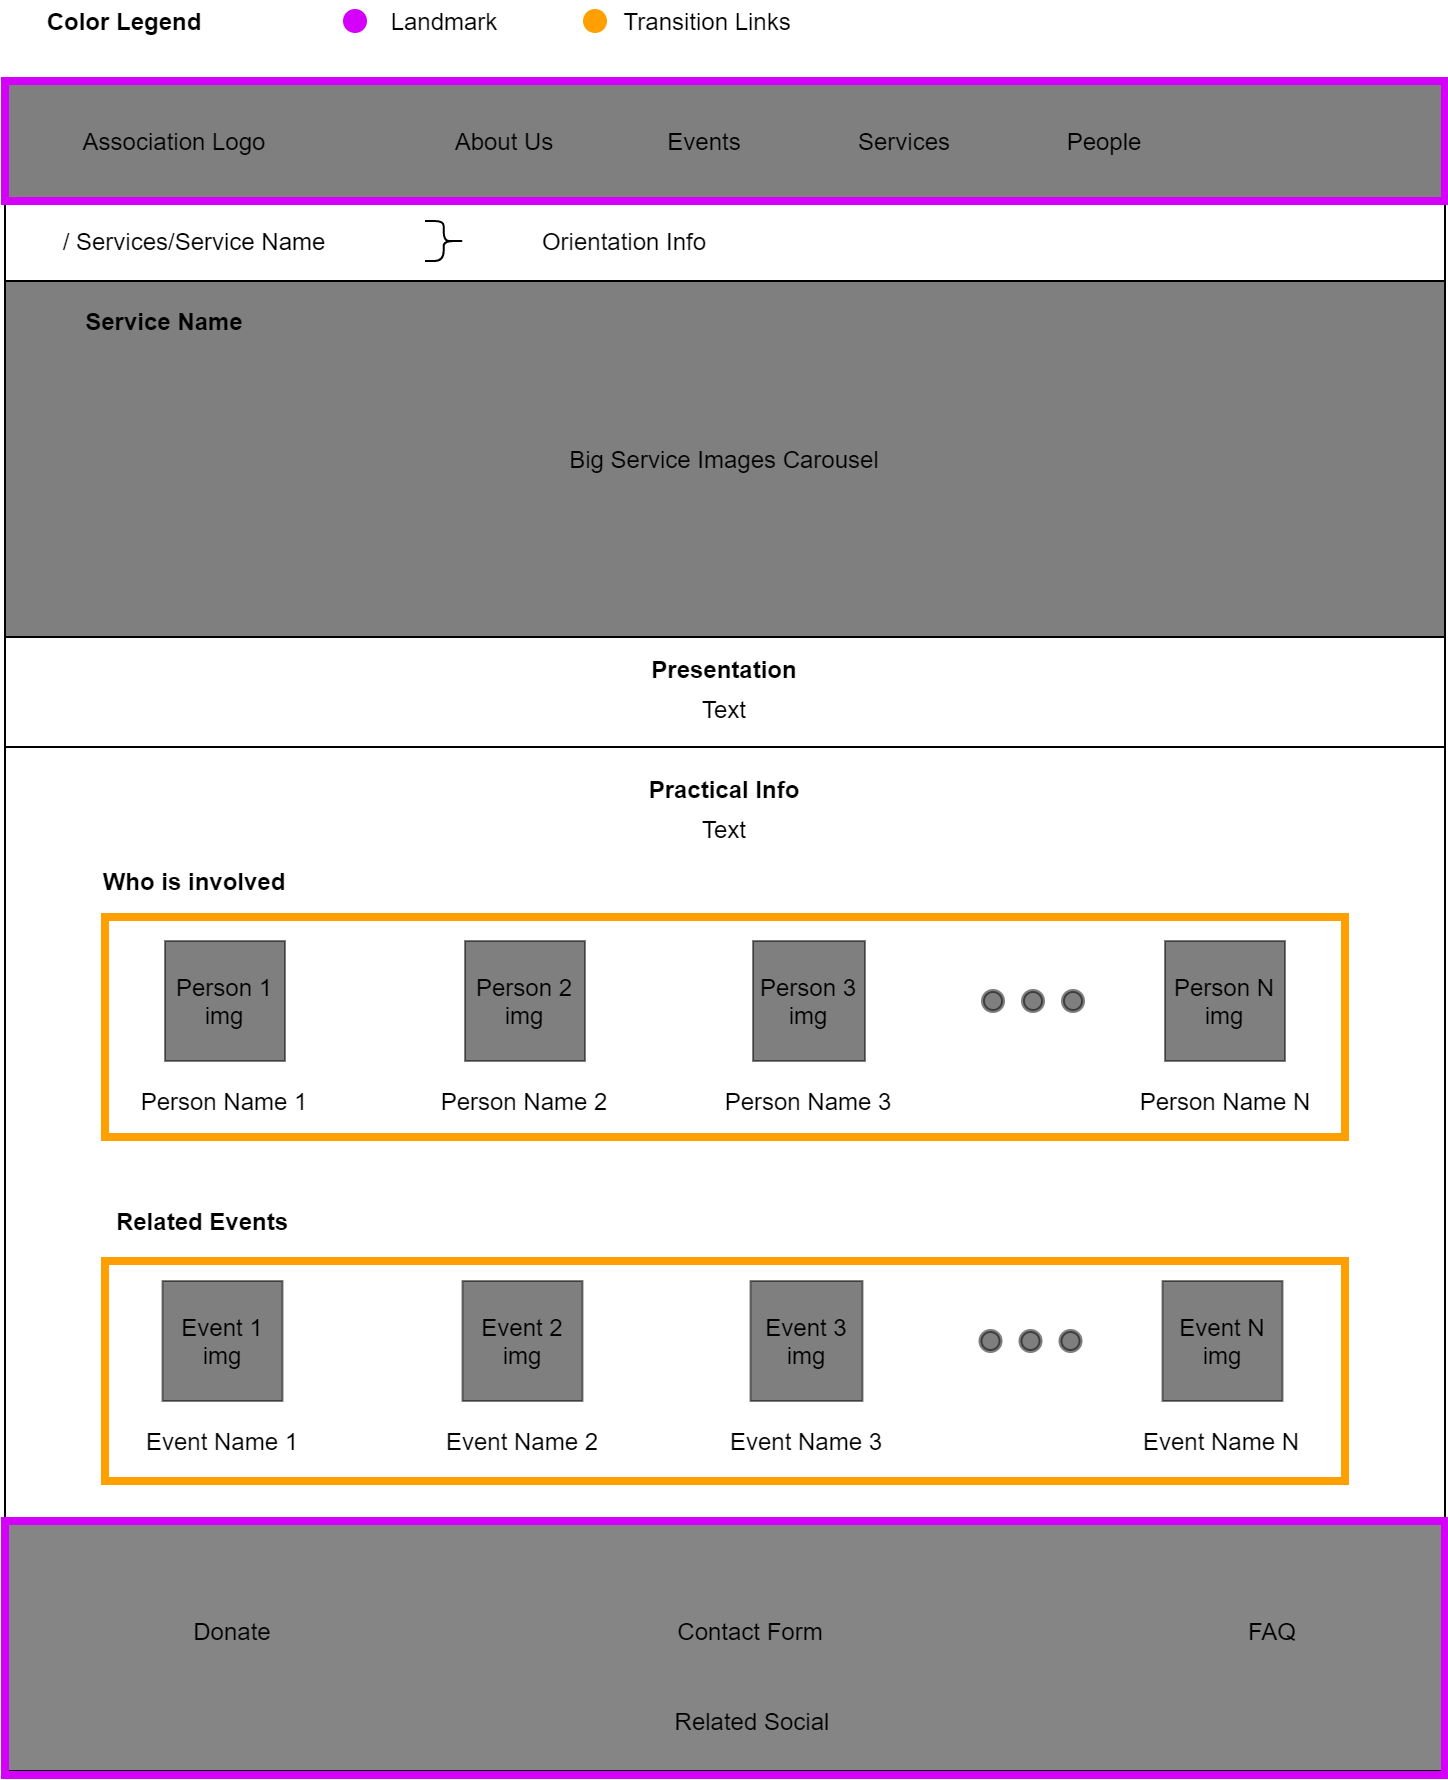
\includegraphics[width=\textwidth]{./assets/servicedetails.png}
			\caption{Service Page - Design in the small}
		\end{minipage}
\end{figure}
\FloatBarrier
